\documentclass[a4paper,10pt]{article}
\usepackage[utf8]{inputenc}
\usepackage{graphicx}
\usepackage{amsmath}
\usepackage{amssymb}
\usepackage{amsthm}
\usepackage{booktabs}
\usepackage{caption}
\usepackage{geometry}
%\usepackage{hyperref}
\usepackage{makeidx}
\usepackage{microtype}
\usepackage{subfig}
\usepackage{tabularx}
\usepackage{url}
\usepackage{varioref}
\usepackage[italian]{babel}
\usepackage{xcolor}
\usepackage{multicol}
\usepackage{mathtools}
\usepackage{booktabs}
\usepackage{gensymb}


\title{Moto di un volano\\
\begin{large}
Dipartimento di Fisica E.Fermi - Università di Pisa
\end{large}}

\author{Di Ubaldo Gabriele}
\date{}

\begin{document}

\maketitle

\tableofcontents

%%%%%%%%%%%%%%%%%%%%%%%%%%%%%%%%%%%%%%%%%%%%%%%%%%%%%%%%%%%%%%%%%%%%%%%%%%%%%%%%%%%%%%%%%%%%%%%%%%%%%%%%%%%%%%%%%%%%%%%%%%%%%%%%%%%%%%%%%%%%%%%%%%%%%%%%%%%%%%%%%%%%%%%%%%%%%%%%%%%
\section{Introduzione}
\subsection{Teoria}
\textbf{Obiettivo:} Misurare il momento della forza di atttrito nel moto di un volano libero e la velocità angolare sotto l'azione di una forza esterna.\\
\textbf{Moto libero:} Lùnica forza esterna è la forza di attrito data dai cuscinetti a sfera che non smorzano l'attrito perfettamente ma ne trasformano gran parte in attrito volvent, significativamente
minore del radente. Per misurare il momento $\tau_{att}$ misuriamo l'accelerazione angolare del moto supponendo che la forza di attrito non dipenda da $\omega$. Nel nostro modello infatti l'atrito da misurare è solo volvente perchè tracuriamo l'attrito viscoso dell'aria proporzionale a $\omega$.
\begin{equation}
 \omega(t)=\omega_0-\frac{\tau_{att}}{I}t
\end{equation}
Il momento d'inerzia di un disco è $\frac{1}{2}mr^2$.

\textbf{Moto forzato:} Le equazioni cardinali del sistema sono le seguenti:
\begin{equation}
 m\ddot{z}=mg-T
\end{equation}

\begin{equation}
 I\alpha=Tr-\tau_{att}
\end{equation}
Siccome il filo è inestensibile la sua accelerazione è uguale a quella del disco:
\begin{equation}
 \ddot{z}=\alpha r
\end{equation}
La soluzione per l'accelerazione angolare è:
\begin{equation}
 \alpha=\frac{\pm mgr-\tau_{att}}{I+mr^2}
\end{equation}
Il + coincide con la discesa $(\alpha>0)$ e il - con la salita $(\alpha<0)$)


\subsection{Apparato sperimentale}
\begin{itemize}
\item{Volano dotato di encoder}
\item{Piattino appeso al volano}
\item{Serie di pesetti}
\item{Programma di acquisizione}
\end{itemize}

%%%%%%%%%%%%%%%%%%%%%%%%%%%%%%%%%%%%%%%%%%%%%%%%%%%%%%%%%%%%%%%%%%%%%%%%%%%%%%%%%%%%%%%%%%%%%%%%%%%%%%%%%%%%%%%%%%%%%%%%%%%%%%%%%%%%%%%%%%%%%%%%%%%%%%%%%%%%%%%%%%%%%%%%%%%%%%%%%%%
\section{Esperimento}
\subsection{Acquisizione misure}
\textbf{Moto libero} Abbiamo dato una spinta iniziale al disco prima senza piattello e poi con per poter verificare se effettivamente il piattello è trascurabile. 
Per misurare la massa del disco abbiamo misurato col calibro le dimensioni del disco, trovato il volume e moltiplicato per la densità dell'alluminio:
il raggio del volano è $r_v=16.1\pm0.1cm$, lo spessore è $h=1.35\pm0.005cm$
Abbiamo pesato il piattello in una bilancia di precisione trovando $m_p=23.224\pm0.001g$.
\\ \textbf{Moto forzato} Il braccio della tensione è $1.28\pm0.03$. Abbiamo misurato la velocità del volano attraverso Arduino e il programma di acquisizione dati Plasduin. Le misure fatte 
corrispondono a pesi di $50, 100, 200, 300, 350 g$ per ognuna delle quali riportiamo il grafico con le misure.
La massa del volano è:
\begin{equation}
V=\pi r_v^2h\rho=2.968kg \quad \Delta V= 2\pi\rho r_vh\Delta r_v+\pi\rho r_v^2\Delta h=0.038kg
\end{equation}

\subsection{Analisi Dati}
Il grafico del moto libero è il seguente:
\pagebreak

 \begin {figure}[!htb]
\begin{center}
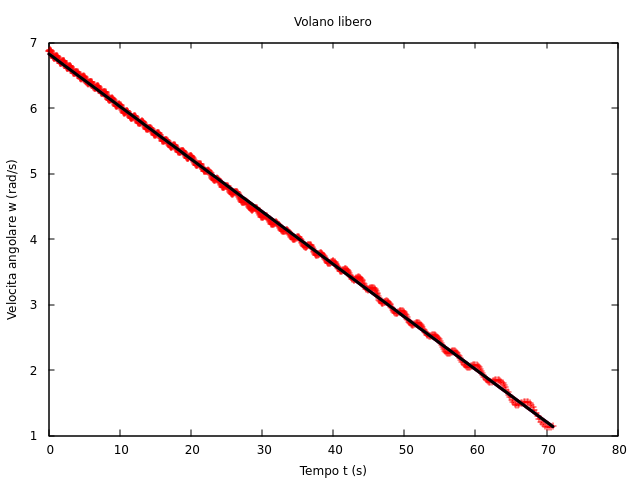
\includegraphics[width=8cm]{/home/zerch/Documents/UNIPI/LAB1/11Volano/dati/volanovuoto.png}
\end{center}
\end{figure}

Il coefficiente della retta best fit è $m=-0.08\pm0.09 \% $ che possiamo moltiplicare per il momento di inerzia per trovare il momento della forza di attrito.
\begin{equation}
\end{equation}
La velocità iniziale è data dall'intersezione con l'asse y cioe $w_0=6.83\pm0.03 \% $. Per il fit si ha $\chi2 =853.18$ e $\chi^2_r=0.95$. Per calcolare $\tau_{att}$ usiamo le seguenti:

\begin{equation}
 \Delta I=\frac{r^2}{2}\Delta m+mr \Delta r \qquad \tau_{att}=-aI \qquad \Delta \tau_{att}=a\Delta I+I\Delta a
\end{equation}
Quindi il momento di inerzia è $I=0.038 \pm0.001kg*m^2$ e otteniamo $\tau_{att}=  0.0030\pm 0.00003 N*m$


Vediamo invece che la presenza del piattello perturba notevolmente il moto del volano in quanto non essendo un peso abbastanza grande, durante il moto tende a oscillare.

 \begin {figure}[!htb]
\begin{center}
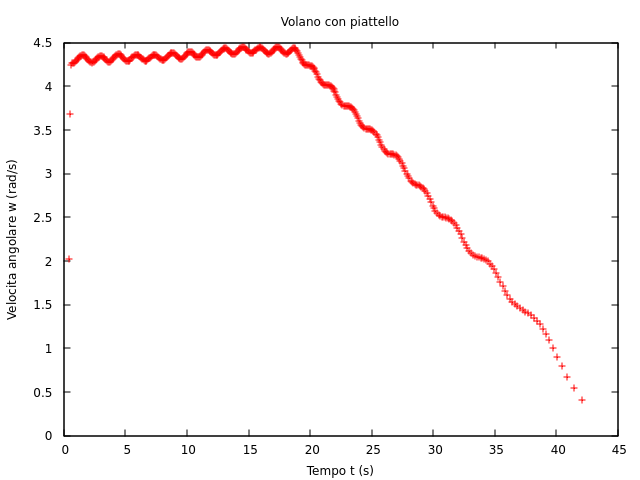
\includegraphics[width=8cm]{/home/zerch/Documents/UNIPI/LAB1/11Volano/dati/volanopiattello1.png}
\end{center}
\end{figure}

I diversi grafici dei moti forzati sono i seguenti:

 \begin {figure}[!htb]
\begin{center}
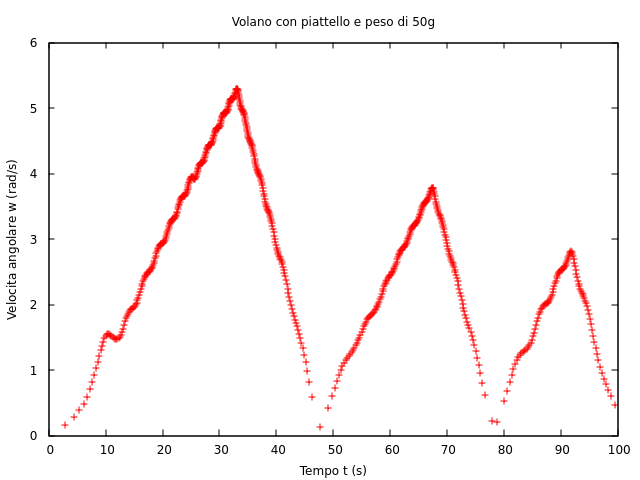
\includegraphics[width=8cm]{/home/zerch/Documents/UNIPI/LAB1/11Volano/dati/volano50.png}
\end{center}
\end{figure}

\begin {figure}[!htb]
\begin{center}
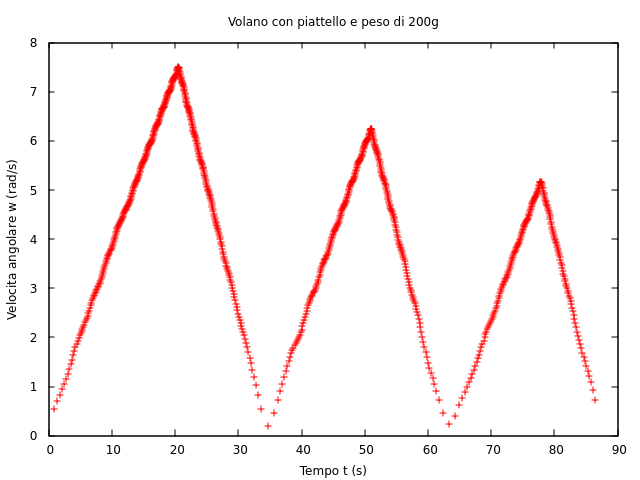
\includegraphics[width=8cm]{/home/zerch/Documents/UNIPI/LAB1/11Volano/dati/volano100.png}
\end{center}
\end{figure}

\begin {figure}[!htb]
\begin{center}
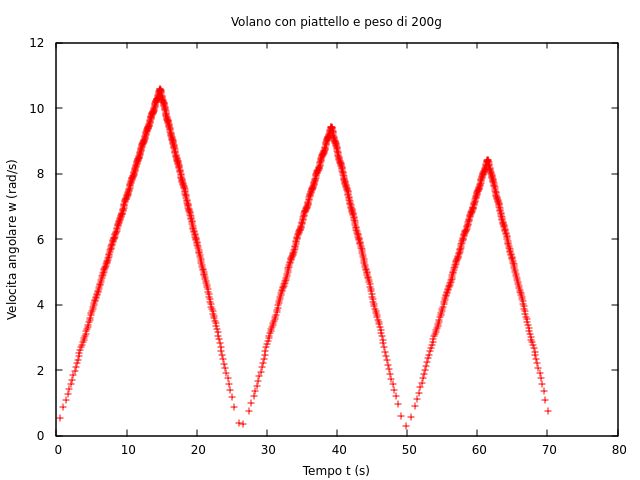
\includegraphics[width=8cm]{/home/zerch/Documents/UNIPI/LAB1/11Volano/dati/volano200.png}
\end{center}
\end{figure} 

\begin {figure}[!htb]
\begin{center}
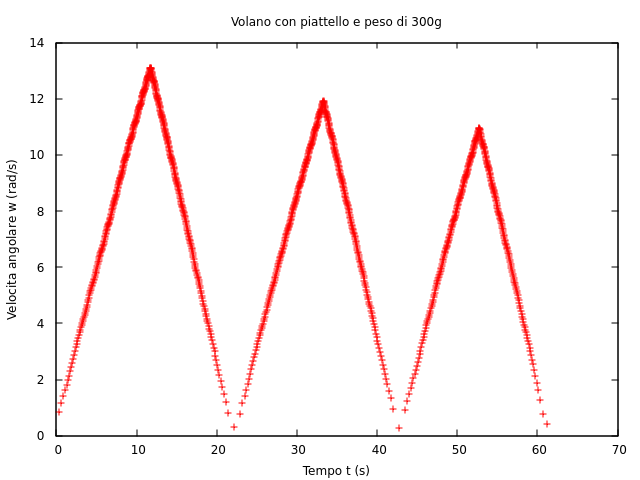
\includegraphics[width=8cm]{/home/zerch/Documents/UNIPI/LAB1/11Volano/dati/volano300.png}
\end{center}
\end{figure}

\begin {figure}[!htb]
\begin{center}
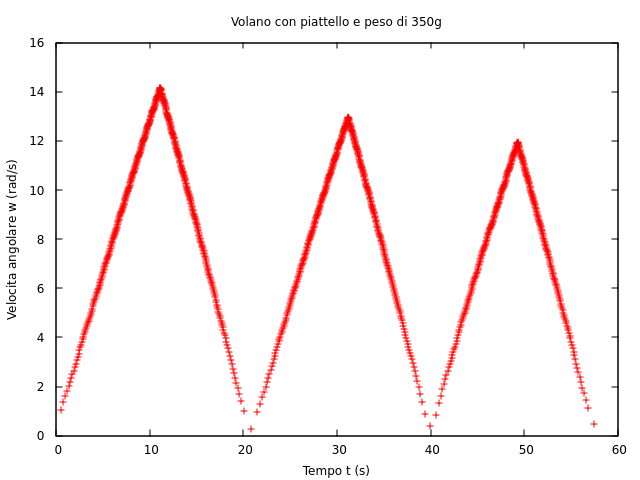
\includegraphics[width=8cm]{/home/zerch/Documents/UNIPI/LAB1/11Volano/dati/volano350.png}
\end{center}
\end{figure}

Possiamo osservare che per $m$ che aumenta i triangoli diventano isosceli cioè la differenza tra il valore assoluto delle pendenze tende a 0 per $m$ che tende a $\infty$:
\begin{equation}
 \lim_{m\to \infty }\alpha_d+\alpha_s= \lim_{m\to \infty }\frac{-2\tau_{att}}{I+mr^2}=0
\end{equation}

Abbiamo preso le misure per $350g$ per la prima discesa e la prima salita e abbiamo fatto il fit per ottenere l'accelerazione angolare in entrambi. I grafici sono i seguenti:
\pagebreak

\begin {figure}[!htb]
\begin{center}
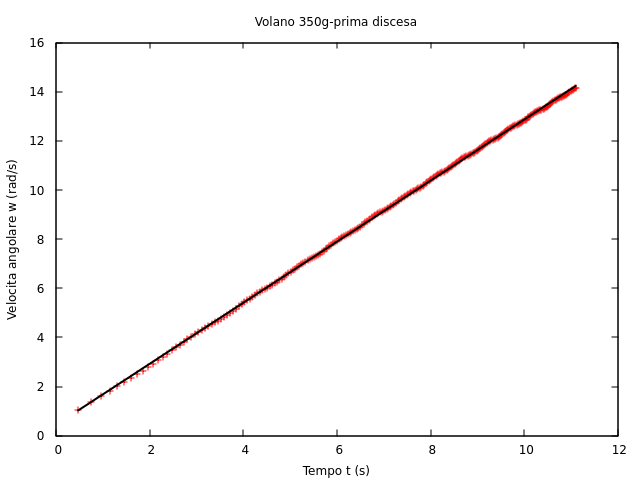
\includegraphics[width=8cm]{/home/zerch/Documents/UNIPI/LAB1/11Volano/dati/volano350part.png}
\end{center}
\end{figure}
L'accelerazione angolare è data dal coefficiente della retta: $\alpha=1.24\pm0.08\%$. Per il fit si ha $\chi^2=297.6$ e $\chi2_r=1.16$.

\begin {figure}[!htb]
\begin{center}
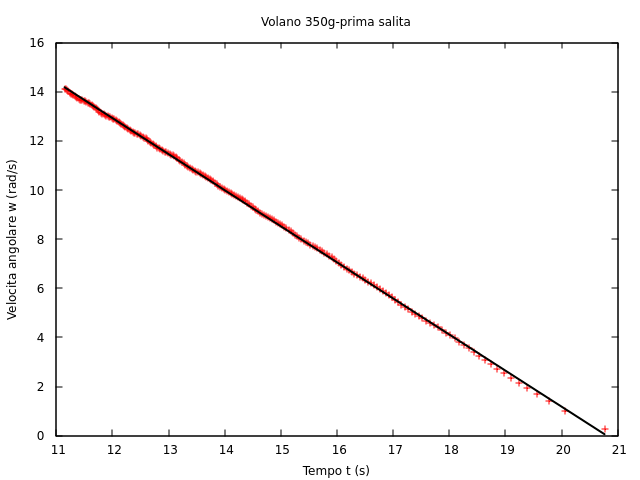
\includegraphics[width=8cm]{/home/zerch/Documents/UNIPI/LAB1/11Volano/dati/volanopart2.png}
\end{center}
\end{figure}
L'accelerazione angolare è data dal coefficiente della retta: $\alpha=-1.47\pm0.11\%$. Per il fit si ha $\chi^2=433.19$ e $\chi2_r=2.00$.
(Se hai voglia potresti fare la differenza tra le accelerazioni per ogni grafico e fittare quei punti con 1/m.)

\pagebreak
\section{Conclusione}
Dato il valore del $\chi^2$ ottenuto possiamo concludere che il nostro modello teorico descrive accuratamente il fenomeno, inoltre il progressivo divenire isosceli dei triangoli è un'altra conferma della validità del nostro modello.

\end{document}


